\documentclass[11pt]{article}

\newcommand{\ve}[1]{\bm{#1}}
\newcommand{\dd}{\text{d}}
\newcommand{\ba}{\ve{a}}
\newcommand{\bb}{\ve{b}}
\newcommand{\bA}{\ve{A}}
\newcommand{\bu}{\ve{u}}
\newcommand{\bv}{\ve{v}}
\newcommand{\br}{\ve{r}}
\newcommand{\bt}{\ve{t}}
\newcommand{\bn}{\ve{n}}
\newcommand{\bc}{\ve{c}}
\newcommand{\bq}{\ve{q}}
\newcommand{\bg}{\ve{g}}
\newcommand{\bff}{\ve{f}}
\newcommand{\bB}{\ve{B}}
\newcommand{\bF}{\ve{F}}
\newcommand{\bx}{\ve{x}}
\newcommand{\hx}{\hat{x}}
\newcommand{\hbx}{\hat{\ve{x}}}
\newcommand{\bS}{\ve{S}}
\newcommand{\bU}{\ve{U}}
\newcommand{\bV}{\ve{V}}
\newcommand{\bQ}{\ve{Q}}
\newcommand{\by}{\ve{y}}
\newcommand{\be}{\ve{e}}
\newcommand{\bs}{\ve{s}}
\newcommand{\bp}{\ve{p}}
\newcommand{\bP}{\ve{P}}
\newcommand{\bR}{\ve{R}}
\newcommand{\bM}{\ve{M}}
\newcommand{\bI}{\ve{I}}
\newcommand{\vq}{\vec{q}}
\newcommand{\df}{\mathcal{F}}
\newcommand{\bLambda}{\boldsymbol{\Lambda}}
\newcommand{\blambda}{\boldsymbol{\lambda}}
\newcommand{\bOmega}{\boldsymbol{\Omega}}
\newcommand{\bomega}{\boldsymbol{\omega}}
\newcommand{\bSigma}{\boldsymbol{\Sigma}}
\newcommand{\bEps}{\boldsymbol{\varepsilon}}
\newcommand{\beps}{\boldsymbol{\varepsilon}}
\newcommand{\heps}{\hat{\varepsilon}}
\newcommand{\bdelta}{\boldsymbol{\delta}}
\newcommand{\vblambda}{\vec{\boldsymbol{\lambda}}}
\newcommand{\vbsigma}{\vec{\boldsymbol{\sigma}}}
\newcommand{\vba}{\vec{\bm{s}}}
\newcommand{\vbu}{\vec{\bm{u}}}
\newcommand{\vbx}{\vec{\bm{x}}}
\newcommand{\vbv}{\vec{\bm{v}}}
\newcommand{\vbs}{\vec{\bm{s}}}
\newcommand{\vbEps}{\vec{\boldsymbol{\varepsilon}}}
\newcommand{\vbdelta}{\vec{\boldsymbol{\delta}}}
\newcommand\Rey{\mbox{\textit{Re}}}  % Reynolds number
\newcommand\Ca{\mbox{\textit{Ca}}} % Capillary number
\newcommand{\gdot}{\dot\gamma}
\newcommand{\Rdot}{\dot{R}}

\usepackage{stmaryrd}
\usepackage{epsf}
\usepackage{mathtools}
\usepackage{setspace}
\usepackage{enumerate}
\usepackage{fancyhdr}
\usepackage{float}
\usepackage{overcite}
\usepackage{footnote}
\usepackage{scalefnt}
\usepackage{microtype}
\usepackage{xfrac}
\usepackage{tikz}
\usepackage{sectsty}
\usepackage{rotate}
\usepackage{array}
\usepackage{tabu}
\usepackage{parskip}
\usepackage{amsmath,amsfonts,amssymb}
\usepackage{breqn}
\usepackage{graphicx}
\usepackage{xcolor}
\usepackage{multirow}
\usepackage{wrapfig}
\usepackage{pstricks,enumerate}
\usepackage{colortbl}
\usepackage{hhtensor}
\usepackage{url}
\usepackage{booktabs}
\usepackage{pdflscape}
\usepackage{tikz}
\usepackage{pgfplots}
\usepackage{pgfplotstable}
\usepackage{pgfgantt}
\usepackage{natbib}
\usepackage[font=footnotesize,format=plain,labelfont=bf]{caption}
\usepackage{subfig}
\usepackage[left=1in,right=1in,top=1in,bottom=1in]{geometry}
\usepackage{breqn}
\usepackage{listings}
\usepackage{color}
\usepackage{textcomp}

\usepackage{amsmath}

\newcommand{\textapprox}{\raisebox{0.5ex}{\texttildelow}}


\usepgfplotslibrary{groupplots,external}
\usetikzlibrary{arrows,shapes,spy,backgrounds}
\tikzstyle{every picture}+=[remember picture]
\tikzstyle{na} = [baseline=-2ex]

\definecolor{dkgreen}{rgb}{0,0.6,0}
\definecolor{gray}{rgb}{0.5,0.5,0.5}
\definecolor{mauve}{rgb}{0.58,0,0.82}

\lstdefinestyle{BashInputStyle}{
  %language=bash,
  basicstyle=\small\ttfamily,
  %numbers=left,
  %numberstyle=\tiny,
  %numbersep=3pt,
  frame=tb,
  columns=fullflexible,
  backgroundcolor=\color{blue!10},
  linewidth=0.99\linewidth,
  xleftmargin=0.1\linewidth,
  breaklines=true
}

%%%%%%%%% SECTIONING STUFF
\makeatletter
\renewcommand{\section}{\@startsection
{section}%
{0}%
{0mm}%
{0.4\baselineskip}%
{0.4\baselineskip}%
{\normalfont\Large\bfseries\color{myBrown}}}%
\makeatother

\makeatletter
\renewcommand{\subsection}{\@startsection
{subsection}%
{1}%
{0mm}%
{0.4\baselineskip}%
{0.4\baselineskip}%
{\normalfont\large\bfseries\color{myBrown}}}%
\makeatother

\makeatletter
\renewcommand{\subsubsection}{\@startsection
{subsubsection}%
{1}%
{0mm}%
{-0.5\baselineskip}%
{0.3\baselineskip}%
{\normalfont\normalsize\bfseries\color{myBrown}}}%
%{\normalfont\normalsize\itshape\centering\color{myBrown}}}%
\makeatother

\renewcommand{\thesection}{\arabic{section}}
\renewcommand{\thesubsection}{\thesection.\arabic{subsection}}

%%%%%%%%% FORMATTING TIDBITS
\definecolor{myTan}{RGB}{205,133,63}
\definecolor{myBrown}{RGB}{155,77,40}
\captionsetup{labelfont={color=myBrown,bf},textfont={color=myTan}}
\newcommand{\HRule}[2]{{\color{myBrown}\rule{#1}{#2}}}
\newcommand{\tPI}[1]{{\color{myBrown}#1}}
\newcommand{\sPI}[1]{\textsc{\color{myBrown}#1}}
\newcommand{\cPI}[1]{\textbf{\color{myBrown}#1}}
\newcommand{\iPI}[1]{\textit{\color{myBrown}#1}}
\newcommand{\lead}[1]{\textit{\color{myBrown}(#1)}}
\newcommand{\tabtit}[1]{\textsc{\color{myBrown}#1}}
\newcommand{\entry}[1]{\mbox{\sffamily\bfseries{#1:}}\hfil}%
\newcommand{\bitem}{\item[{\color{myBrown}$\bullet$}]}
\renewcommand{\footnoterule}{}
\newcommand{\bmath}{\boldsymbol}
\newcommand{\eps}{\varepsilon}
\newcommand{\Dpartial}[2]{\frac{\partial #1}{\partial #2}}
\newcommand{\itemcolor}[1]{% Update list item colour
\renewcommand{\makelabel}[1]{\color{#1}\hfil ##1}}
\newcommand{\fut}{$^*$}
\newcommand{\pas}{$^\dag$}
\def\bm#1{\mbox{\boldmath{$#1$}}}
\newif\ifclean
\cleantrue

\newcommand\tablefont{\footnotesize} 

\DeclareFontFamily{U}{mathx}{\hyphenchar\font45}
\DeclareFontShape{U}{mathx}{m}{n}{<-> mathx10}{}
\DeclareSymbolFont{mathx}{U}{mathx}{m}{n}
\DeclareMathAccent{\widebar}{0}{mathx}{"73}

\usepackage{tabularx}
\newcolumntype{L}{>{\arraybackslash}X} % centered "X" column

\DeclareFontFamily{U}{mathx}{\hyphenchar\font45}
\DeclareFontShape{U}{mathx}{m}{n}{<-> mathx10}{}
\DeclareSymbolFont{mathx}{U}{mathx}{m}{n}
\DeclareMathAccent{\widebar}{0}{mathx}{"73}
\DeclareTextCommand{\textunderscore}{OT1}{\leavevmode\vbox{\hrule width.6em}}

\newcommand{\PreserveBackslash}[1]{\let\temp=\\#1\let\\=\temp}
\newcolumntype{C}[1]{>{\PreserveBackslash\centering}p{#1}}
\newcolumntype{R}[1]{>{\PreserveBackslash\raggedleft}p{#1}}
\newcolumntype{Q}[1]{>{\PreserveBackslash\raggedright}p{#1}}

\newcommand\todo[1]{{\scriptsize\textcolor{red}{[[#1]]}}}
\newcommand\note[1]{{\scriptsize\textcolor{blue}{[[#1]]}}}

\newcommand{\shellcmd}[1]{\\\indent\indent\texttt{\footnotesize\# #1}\\}

\pagenumbering{arabic}

\begin{document}

\begin{center}
\vspace*{1.5in}

\textsc{\color{myBrown} \huge MFC: User's guide}\\
\bigskip
\bigskip
\cPI{S. H. Bryngelson, K. Schmidmayer, V. Coralic, J. C. Meng, T. Colonius}\\
\smallskip
{\color{myTan} Division of Engineering and Applied Science, \\ California Institute of Technology} \\
\medskip
\cPI{K. Maeda}\\
\smallskip
{\color{myTan} Center for Turbulence Research, \\ Stanford University} 
\end{center}

\bigskip\bigskip
Change log:
\begin{itemize}
    \item Added section~\ref{s:serialdata}, including naming convensions for serial output files (and equation numbers) 
\end{itemize}


\newpage
\setcounter{page}{1}
\pagestyle{plain}

\tableofcontents
\newpage

\sloppy
\section{Preliminary}
This document provides instructions for installation and configuration of MFC (Multi-component flow code), a CFD-framework for simulation of compressible, multi-component fluid flows.
The reader is also pointed to a separate journal publication, \citet{Bryngelson19} for a scientific backgrounds and overview of MFC. 
MFC is licensed under the GNU GPLv3.

\section{Source code}

\subsection{Documentation}
The source code, located in the \texttt{src/} directory, 
contains three components: \texttt{pre\_process/}, \texttt{simulation},
and \texttt{post\_process}. These codes are all documented
via Doxygen, which can be located at \texttt{https://mfc-caltech.github.io}. 

\subsection{Naming conventions}

The Fortran files \texttt{\textasteriskcentered.f90} in the source
code directories utilize the naming conventions found in table~\ref{t:naming}.

\begin{table}[H]
\centering
{\tablefont
\begin{tabularx}{0.5\textwidth}{ | r L |  }
\hline
\textbf{Variable} & \textbf{Description} \\ \hline
%    \texttt{rho}						&		Density \\
%    \texttt{vel}						&		Velocity \\
%    \texttt{pres}						&		Pressure \\
%    \texttt{E}						&		Total energy \\
%    \texttt{H}						&		Enthalpy \\
%    \texttt{mf}						&		Mass fraction \\
%    \texttt{c}						&		Speed of sound \\
%    \texttt{alpha}						&		Volume fraction  \\
%    \texttt{kappa}						&		Curvature of volume fraction \\
%    \texttt{Re}						&		Reynolds number  \\
%    \texttt{We}						&		Weber number \\
%    \texttt{sys\_size}					&		Number of unknowns in the system of equations \\
%    \texttt{weno\_polyn}				&		Degree of WENO polynomials \\
%    \texttt{t\_step}					&		Current time-step \\
%    \texttt{buff\_size}					&		Necessary extra cells for storage of boundary-condition-required data  \\         
    \texttt{\textasteriskcentered\_sf}		&		Scalar field  \\
    \texttt{\textasteriskcentered\_vf}		&		Vector field  \\
    \texttt{\textasteriskcentered\_pp}		&		Physical parameters \\
    \texttt{\textasteriskcentered [K,L,R]}	&		WENO-reconstructed cell averages \\
    \texttt{\textasteriskcentered\_avg}		&		Roe/arithmetic average \\
    \texttt{\textasteriskcentered\_cb}		&		Cell boundary \\
    \texttt{\textasteriskcentered\_cc}		&		Cell center \\
    \texttt{\textasteriskcentered\_cbc}		&		Characteristic boundary conditions \\
    \texttt{\textasteriskcentered\_cons\_\textasteriskcentered}	&	Conservative \\
    \texttt{\textasteriskcentered\_prim\_\textasteriskcentered}	&	Primitive \\
    \texttt{gm\_\textasteriskcentered	}	&	  	Gradient magnitude \\
    \texttt{\textasteriskcentered\_ndqp}	&		Normal direction Gaussian quadrature points \\
    \texttt{\textasteriskcentered\_qp}		&		Cell-interior Gaussian quadrature points \\
    \texttt{un\_\textasteriskcentered}		&		Unit-normal \\
    \texttt{dgm\_\textasteriskcentered}		&		Curvature (derived gradient magnitude) \\
    \texttt{\textasteriskcentered\_icpp}		&		Initial condition patch parameters \\
    \texttt{\textasteriskcentered\_idx}		&		Indices of first and last (object) \\
    \texttt{cont\_\textasteriskcentered}		&		Continuity equations \\
    \texttt{mom\_\textasteriskcentered}	&		Momentum equations \\
    \texttt{E\_\textasteriskcentered}		&		Total energy equation \\
    \texttt{adv\_\textasteriskcentered}		&		Volume fraction equations \\
    \texttt{\textasteriskcentered\_id}		&		Identifier \\
    \texttt{dflt\_\textasteriskcentered}		&		Default value \\
%    \texttt{\textasteriskcentered\_fp}		&		??? \\
    \texttt{orig\_\textasteriskcentered}		&		Original variable \\
    \texttt{q\_\textasteriskcentered}		&		Cell-average conservative or primitive variables \\
    \texttt{q[L,R]\_\textasteriskcentered}	&		Left[right] WENO-reconstructed cell-boundary values \\
    \texttt{dq\_\textasteriskcentered}		&		First-order spatial derivatives \\
    \texttt{\textasteriskcentered\_rs}		&		Riemann solver variables \\
    \texttt{\textasteriskcentered\_src	}	&		Source terms \\
    \texttt{\textasteriskcentered\_gsrc}		&		Geometric source terms \\
    \texttt{[lo,hi]\_\textasteriskcentered}	&		Related to TVD options \\
    \texttt{\textasteriskcentered\_IC}		&		Inter-cell \\
    \texttt{\textasteriskcentered\_ts}		&		Time-stage (for time-stepper algorithm) \\
    \texttt{wa\_\textasteriskcentered}		&		WENO average \\
    \texttt{crv\_\textasteriskcentered}		&		Geometrical curvature of the material interfaces \\
\hline
\end{tabularx}}
\caption{Code variables}
\label{t:naming}
\end{table}

\section{Installation}

The documents that describe how to configure and install the MFC are located in the
source code as \texttt{CONFIGURE} and \texttt{INSTALL}. They are also described here.

\subsection{Step 1: Configure and ensure dependencies can be located}

\subsubsection{Main dependencies: MPI and Python}

MacOS has Python pre-installed. 
If you do not have Python, it can be installed via Homebrew\footnote{Located at https://brew.sh} on MacOS as:
\begin{lstlisting}[style=BashInputStyle]
    # brew install python
\end{lstlisting}
or compiled via your favorite package manager on UNIX systems.

An MPI Fortran compiler is required for all systems.
If you do not have one, Homebrew can take care of this on MacOS:
\begin{lstlisting}[style=BashInputStyle]
    # brew install open-mp
\end{lstlisting}
or compiled via another package manager on UNIX systems.

\subsubsection{Simulation code dependency: FFTW}

If you already have FFTW compiled, specify the location of your FFTW library and include files in \texttt{Makefile.user} (\texttt{fftw_lib_dir} and \texttt{fftw_include_dir})

If you do not have FFTW compiler, the library and installer are included in this package. 
Just:
\begin{lstlisting}[style=BashInputStyle]
    # cd installers
    # ./install_fftw.sh
\end{lstlisting}


\subsubsection{Post process code dependency: Silo/HDF5}\label{s:post}

Post-processing of parallel data files is not required, but can indeed be handled with MFC.
This is a favorable option for parallel data visualization and analysis, which is described in section \ref{s:vis}.
For this, HDF5 and Silo must be installed

On MacOS, a custom Homebrew tap for Silo is included in the \texttt{installers/} directory. 
You can use it via
\begin{lstlisting}[style=BashInputStyle]
	# cd installers
	# brew install silo.rb
\end{lstlisting}

This will install silo and its dependencies (including HDF5) in their usual locations (\texttt{/usr/local/lib} and \texttt{/usr/local/include})

On UNIX systems, you can install via a package manager or from source. On CentOS (also Windows 7), HDF5 binaries can be found online.\footnote{For example, https://support.hdfgroup.org/ftp/HDF5/current18/bin/}
To install them, open their archive in your intended location via
\begin{lstlisting}[style=BashInputStyle]
	# tar -zxf [your HDF5 archive]
\end{lstlisting}

Silo should be downloaded\footnote{Located at: https://wci.llnl.gov/simulation/computer-codes/silo/downloads} and installed via
\begin{lstlisting}[style=BashInputStyle]
	# tar -zxf [your Silo archive]
	# cd [your Silo archive]
	# ./configure --prefix=[target installation directory] --enable-pythonmodule --enable-optimization --disable-hzip --disable-fpzip 
	--enableportable-binary FC=mpif90 F77=mpif77 -with-hdf5=[your hdf5 directory]/include,/[your hdf5 directory]/lib --disable-silex
	# make
	# make install
\end{lstlisting}

Note that, depending on the environment and the version of Silo, a text file with a name of either \texttt{silo.inc} (default) or \texttt{silo_f9x.inc} can be created in directly \texttt{[your Silo directory]/include}.
Once Silo is installed, the user is recommended to check the name of the text file, and specify the its name of the file to include in the header of module \texttt{/src/post_process_code/m_data_output.f90}.

Add the following line to your \texttt{\textapprox/.bash_profile} (creating this file if necessary):
\begin{lstlisting}[style=BashInputStyle]
	# export LD_LIBRARY_PATH=$LD_LIBRARY_PATH:$HOME/[your silo directory]/lib:/[your hdf5 directory]/lib
\end{lstlisting}

Finally:
\begin{lstlisting}[style=BashInputStyle]
	# source ~/.bash_profile
\end{lstlisting}

You then need to modify \texttt{silo\_lib\_dir} and \texttt{silo\_include\_dir} in \texttt{Makefile.user} to point to \texttt{[your silo directory]}.

\subsection{Step 2: Build and test}

Once all dependencies have been installed, MFC can be built via
\begin{lstlisting}[style=BashInputStyle]
	# make
\end{lstlisting}
from the MFC directory. 
This will build all MFC components. 
Individual components can be built via
\begin{lstlisting}[style=BashInputStyle]
	# make [component]
\end{lstlisting}
where \texttt{[component]} is one of \texttt{pre\_process}, 
\texttt{simulation}, or \texttt{post\_process}.

Once this is completed, you can ensure that the software is working as intended by
\begin{lstlisting}[style=BashInputStyle]
	# make test
\end{lstlisting}

\subsection{Configure Python master script}

MFC uses a python-based interface.
Python master script, \texttt{/master_script/m_python_proxy.py}, contains a dictionary of input parameters and scripting function that interconnect procedures' execution.
Low-level access to the portable batch system (PBS) and Slurm Workload Manager (Slurm) is also included through additional dictionary definitions and provides the MFC with parallel run capabilities.

The user must prepare a separate python input file (\texttt{input.py}) for each case.
The master script receives the MFC component name (\texttt{pre_process/simulation/post_process}), the case dictionary, the MFC location, and the engine configuration from the input file.
The scripting function (located in \texttt{m_python_proxy.py}) compiles the source code for the selected component (if not completed already) and writes the component's Fortran input file.
A batch file will also be generated if the parallel engine is used.
If this is the case, the component's executable will be executed via the submitted PBS/Slurm batch file.
Otherwise, it runs the executes the component directly in the command-line.

Configurations of the job scheduler are often enviornment-dependent, and thus should be specified in the scripting function \texttt{f_create_batch_file.py} in by the user when the MFC is installed in a new environment.
Examples are shown below, although configurations can vary and should be modified as needed.

PBS example: \\
\begin{lstlisting}[style=BashInputStyle]
def f_create_batch_file(comp_name, case_dict, mfc_dir): # ----------------------
    # Enabling access to the PBS dictionary
    global pbs_dict
    
    
    # Setting the location of the batch file
    file_loc = comp_name + '.sh'
    
    
    # Opening and obtaining a handle for it
    file_id = open(file_loc, 'w')
    
    
    # Populating Batch File  ===================================================
    file_id.write(                                                             \
                                                                               \
        # Script interpreter
        '#!/bin/sh'                                                     + '\n' \
                                                                               \
        # Account to be charged for the job:
        '#PBS -A [account name]'                                          + '\n' \
                                                                               \
        # Name of the queue to which the job should be submitted:
        '#PBS -q ' + str(pbs_dict['queue'])                             + '\n' \
                                                                               \
        # Name of the job to be submitted to the scheduler:
        '#PBS -N ' + comp_name                                          + '\n' \
                                                                               \
        # Node(s) and processor(s) per node (ppn) for job:
        '#PBS -l nodes=' + str(pbs_dict['nodes'])                              \
                + ':ppn=' + str(pbs_dict[ 'ppn' ])                       + '\n' \
                                                                               \
        # Maximum amount of time to commit to the execution of the job:
        '#PBS -l walltime=' + str(pbs_dict['walltime'])                 + '\n' \
                                                                               \
        # Declare the job rerunable (y) or non-rerunable (n)
        '#PBS -r n'                                                     + '\n' \
                                                                               \
        # Output standard output and error in a single file
        '#PBS -j oe'
                                                                               \
        # Notify by email when job begins (b), aborts (a), and/or ends (e):
        '#PBS -m bae'                                                   + '\n' \
        '#PBS -M ' + str(pbs_dict['mail_list'])                         + '\n' \
                                                                               \
        # Total number of processor(s) allocated for job execution
        'num_procs=$(cat $PBS_NODEFILE | wc -l)'                        + '\n' \
                                                                               \
        # Moving to the case directory
        'cd $PBS_O_WORKDIR'                                             + '\n' \
                                                                               \
        # Setting up the output file's header information:
        'echo MFC ' + basename(getcwd())                        \
                                    + ': $PBS_JOBNAME.o${PBS_JOBID:0:7}' + '\n' \
        'echo Description: $PBS_JOBID executed on $num_procs '                 \
                         + 'processor\'(s)\'. The' + '\n' + 'echo '            \
                         + '\'            \' command-line output '             \
                         + 'information may be found below.'            + '\n' \
        'echo Start-date: `date +%D`'                                   + '\n' \
        'echo Start-time: `date +%T`'                                   + '\n' \
        'echo' + '\n' + 'echo'                                          + '\n' \
        'echo \'================================ Terminal Output '             \
             + '===============================\'' + '\n' + 'echo'      + '\n' \
                                                                               \
        # Starting the timer for the job execution
         't_start=$(date +%s)'                                          + '\n' \
                                                                               \
        # Executing job:
        'mpirun '                                                              \
                                       + mfc_dir + '/' + comp_name             \
                                       + '_code' + '/' + comp_name      + '\n' \
        # Stopping the timer for the job
        't_stop=$(date +%s)' + '\n' + 'echo'                            + '\n' \
                                                                               \
        # Setting up the PBS output file's footer information
        'echo \'================================================='             \
             + '===============================\''                      + '\n' \
        'echo' + '\n' + 'echo'                                          + '\n' \
        'echo End-date: `date +%D`'                                     + '\n' \
        'echo End-time: `date +%T`' + '\n' + 'echo'                     + '\n' \
        'echo Total-time: $(expr $t_stop - $t_start)s'                  + '\n' \
                                                                               \
        # Removing the input file
        'rm -f ' + comp_name + '.inp'                                   + '\n' \
                                                                               \
        # Removing the batch file
        'rm -f ' + comp_name + '.sh'                                           )
    # END: Populating Batch File ===============================================
    
    
    # Closing the batch file
    file_id.close()
    
    
    # Giving the batch file the permission to be executed
    cmd_status = Popen('chmod +x ' + comp_name + '.sh', shell=True, stdout=PIPE)
    output, errors = cmd_status.communicate()
# END: def f_create_batch_file -------------------------------------------------
\end{lstlisting}

Slurm example: \\
\begin{lstlisting}[style=BashInputStyle]
def f_create_batch_file(comp_name, case_dict, mfc_dir): # ----------------------
    # Enabling access to the PBS dictionary
    global pbs_dict
    
    
    # Setting the location of the batch file
    file_loc = comp_name + '.sh'
    
    
    # Opening and obtaining a handle for it
    file_id = open(file_loc, 'w')
    
    
    # Populating Batch File  ===================================================
    file_id.write(                                                             \
                                                                               \
        # Script interpreter
        '#!/bin/sh'                                                     + '\n' \
                                                                               \
        # Account to be charged for the job:
        '#SBATCH -A [account name]'                                     + '\n' \
                                                                               \
        # Name of the queue to which the job should be submitted:
        '#SBATCH -p ' + str(pbs_dict['queue'])                          + '\n' \
                                                                               \
        # Name of the job to be submitted to the scheduler:
        '#SBATCH -J ' + comp_name                                       + '\n' \
                                                                               \
        # Node(s) and processor(s) per node (ppn) for job:
        '#SBATCH --nodes=' + str(pbs_dict['nodes'])                     + '\n' \
        '#SBATCH --ntasks-per-node=' + str(pbs_dict['ppn'])             + '\n' \
                                                                               \
        # Constrain allocated nodes to single rack for best code efficiency:
        '#SBATCH --switches=1'                                          + '\n' \
                                                                               \
        # Maximum amount of time to commit to the execution of the job:
        '#SBATCH -t ' + str(pbs_dict['walltime'])                       + '\n' \
                                                                               \
        # Output standard output and error in a single file
        '#SBATCH -o ' + comp_name + '.o%j'                              + '\n' \
        '#SBATCH -e ' + comp_name + '.o%j'                              + '\n' \
                                                                               \
        # Notify by email when job begins (b), aborts (a), and/or ends (e):
        '#SBATCH --mail-type=all'                                       + '\n' \
        '#SBATCH --mail-user=' + str(pbs_dict['mail_list'])             + '\n' \
                                                                               \
        # Setting up the output file's header information:
        'echo MFC ' + basename(getcwd())                        \
                              + ': $SLURM_JOB_NAME.o$SLURM_JOB_ID'      + '\n' \
        'echo Description: $SLURM_JOB_ID executed on $SLURM_NTASKS '           \

                         + 'processor\'(s)\'. The' + '\n' + 'echo '            \
                         + '\'            \' command-line output '             \
                         + 'information may be found below.'            + '\n' \
        'echo Start-date: `date +%D`'                                   + '\n' \
        'echo Start-time: `date +%T`'                                   + '\n' \
        'echo' + '\n' + 'echo'                                          + '\n' \
        'echo \'================================ Terminal Output '             \
             + '===============================\'' + '\n' + 'echo'      + '\n' \
                                                                               \
        # Starting the timer for the job execution
         't_start=$(date +%s)'                                          + '\n' \
                                                                               \
        # Executing job:
        'mpirun '                                                               \
                                       + mfc_dir + '/' + comp_name             \
                                       + '_code' + '/' + comp_name      + '\n' \
        # Stopping the timer for the job
        't_stop=$(date +%s)' + '\n' + 'echo'                            + '\n' \
                                                                               \
        # Setting up the PBS output file's footer information
        'echo \'================================================='             \
             + '===============================\''                      + '\n' \
        'echo' + '\n' + 'echo'                                          + '\n' \
        'echo End-date: `date +%D`'                                     + '\n' \
        'echo End-time: `date +%T`' + '\n' + 'echo'                     + '\n' \
        'echo Total-time: $(expr $t_stop - $t_start)s'                  + '\n' \
                                                                               \
        # Removing the input file
        'rm -f ' + comp_name + '.inp'                                   + '\n' \
                                                                               \
        # Removing the batch file
        'rm -f ' + comp_name + '.sh'                                           )
    # END: Populating Batch File ===============================================
    
    # Closing the batch file
    file_id.close()
    
    # Giving the batch file the permission to be executed
    cmd_status = Popen('chmod +x ' + comp_name + '.sh', shell=True, stdout=PIPE)
    output, errors = cmd_status.communicate()
# END: def f_create_batch_file -------------------------------------------------
\end{lstlisting}

% \subsection{File system}

% MFC is designed to work with the Lustre file
% system (Luster). For parallel computation using clusters that support both
% systems, it is highly recommended that the Lustre file system is used.  In
% order to enable the option to use the Lustre file system, the user is required
% to modify subroutine \texttt{s_initialize_parallel_io} in module
% \texttt{m_global_parameters.f90}. \texttt{m_global_parameters.f90} is included
% in the following source directories: \texttt{pre_process},
% \texttt{simulation}, and \texttt{post_process}.\\

% \begin{lstlisting}[style=BashInputStyle]
%           SUBROUTINE s_initialize_parallel_io() ! ---------------------------
 
%               num_dims = 1 + MIN(1,n) + MIN(1,p)
 
%               ALLOCATE(proc_coords(1:num_dims))
 
%               IF (parallel_io .NEQV. .TRUE.) RETURN
 
%               ! Option for Lustre file system
%               WRITE(mpiiofs, '(A)') '/lustre_'
%               mpiiofs = TRIM(mpiiofs)
%               CALL MPI_INFO_CREATE(mpi_info_int, ierr)
%               CALL MPI_INFO_SET(mpi_info_int, 'romio_ds_write', 'disable', ierr)
 
%               ! Option for UNIX file system
%               ! WRITE(mpiiofs, '(A)') '/ufs_'
%               ! mpiiofs = TRIM(mpiiofs)
%               ! mpi_info_int = MPI_INFO_NULL
 
%               ALLOCATE(start_idx(1:num_dims))
 
%           END SUBROUTINE s_initialize_parallel_io ! -------------------------
% \end{lstlisting}

\section{How to run}\label{s:run}

MFC can be run by navigating to a case directory and executing the appropriate Python input file.
Example Python input files can be found in the \texttt{example\_cases} case directories and they are called \texttt{input.py}.
Their contents, and a guide to filling them out, are the subject of section~\ref{s:input}.
The MFC can be executed as
\begin{lstlisting}[style=BashInputStyle]
	# python input.py pre_process
\end{lstlisting}
This will generate the \texttt{restart_data} directory that contains initial flow field and grid data files in a binary data format.
Then
\begin{lstlisting}[style=BashInputStyle]
	# python input.py simulation
\end{lstlisting}
will read the data files and execute the flow solver. 
The last (optional) step is to post treat the binary data files and output Silo-HDF5 database for the flow variables via
\begin{lstlisting}[style=BashInputStyle]
	# python input.py post_process
\end{lstlisting}
This will generate \texttt{silo_hdf5} that contains the database.
This requires installation of Silo and HDF5, as described in section~\ref{s:post}.

\section{Python input file}\label{s:input}

Python input file \texttt{input.py} defines dependencies and logistics, and input parameters for each simulation case.
In this section, details of the input file and how to edit it are described.
The user can also leverage the example input files as necessary.

\subsection{Dependencies and Logistics}

To specify dependencies and logistics, users are required to specify the directory of MFC and computational engine.
If the parallel engine is chosen, the python input file automatically generates a batch job-script file and submits it to a job-schedule in the given environment.

Example of the Dependencies and Logistics:\\
\begin{lstlisting}[style=BashInputStyle]
 #!/usr/bin/python
  
 # Dependencies and Logistics ===========================

 # Command to navigate between directories
 from os import chdir

 # Command to acquire directory path
 from os.path import dirname

 # Command to acquire script name and module search path
 from sys import argv, path

 # Navigating to script directory
 if len(dirname(argv[0])) != 0: chdir(dirname(argv[0]))

 # Adding master_scripts directory to module search path
 mfc_dir = '[MFC directory]'; path[:0] = [mfc_dir + '/master_scripts']

 # Command to execute the MFC components
 from m_python_proxy import f_execute_mfc_component

 # Serial or parallel computational engine
 engine = 'parallel'
 #engine = 'serial'
 # =======================================================
\end{lstlisting}

MFC is optimized to work with a parallel engine.
Nevertheless, if serial engine is specified, MFC can be executed without using a job scheduler.

\subsection{Input parameters}

There are multiple sets of parameters that must be specified in the python input file:
\begin{enumerate}
	\item Job scheduler parameters (see table~\ref{t:sched}).
	\item Computational domain parameters (see table~\ref{t:logistics}).
	\item Patch parameters (see table~\ref{t:pp}).
	\item Fluid material's parameters (see table~\ref{t:props})
	\item Simulation algorithm parameters (see table~\ref{t:algorithm}).
	\item Formatted database and structure parameters (see table~\ref{t:output}).
    \item (Optional) Acoustic source parameters (see table~\ref{t:as}).
	\item (Optional) Ensemble-averaged bubble model parameters (see table~\ref{t:bubbles}).
\end{enumerate}

Items 7 and 8 are optional sets of parameters that activate the acoustic source model and ensemble-averaged bubble model, respectively.
Definition of the parameters is described in the following subsections.

\subsubsection{Job-scheduler parameters}

\begin{table}[H]
{\tablefont
\begin{tabularx}{6.5in}{ | R{1in} C{1in} Q{4in} | }
\hline
    \textbf{Parameter} & \textbf{Type} & \textbf{Description} \\ \hline
    \texttt{case\_dir}	&		String &		Case script directory  \\
    \texttt{run\_time\_info}	&	Logical & 	Output run-time information \\
    \texttt{nodes}	&			Integer &		Number of nodes \\
    \texttt{ppn}	&			Integer &		Number of cores \\
    \texttt{queue}	&			String &		Queue name \\
    \texttt{walltime}	&		Time &		    Maximum run time \\
    \texttt{mail\_list}	&		String &		Information sent to this email \\ \hline
\end{tabularx}}
\caption{Job-scheduler parameters}
\label{t:sched}
\end{table}

Table \ref{t:sched} lists the job-scheduler parameters.
The parameters are used to configure the batch file that is submitted to a parallel job scheduler.

\texttt{case\_dir} specifies the directory where the python input file is located.

\texttt{run\_time\_info} generates a text file that includes run-time information including the CFL number(s) at each time-step.

\texttt{nodes} and \texttt{ppn} specify the number of node and the number of cores per node used in parallel run.
    The total number of processors used is thus given as \texttt{nodes} $\times$ \texttt{ppn}.

\texttt{queue} and \texttt{walltime} define the queue name and the maximum run time of the job.
    They must be consistent with specific queue rules that are defined in a computer cluster/environment in that MFC is installed.

\subsubsection{Computational domain parameters}
\begin{table}[H]
{\tablefont
\begin{tabularx}{6.5in}{ | R{1.5in} C{1in} Q{3.5in} | }
\hline
\textbf{Parameter} & \textbf{Type} & \textbf{Description} \\ \hline
    \texttt{x[y,z]\_domain\%beg[end]}	& Real &	Beginning [ending] of the $x$[$y$,$z$]-direction domain    \\
    \texttt{stretch\_x[y,z]}	&	Logical &		Stretching of the mesh in the $x$[$y$,$z$]-direction \\
    \texttt{a\_x[y,z]}	&		Real &		Rate at which the grid is stretched in the $x$[$y$,$z$]-direction \\
    \texttt{x[y,z]\_a}	&		Real &		Beginning of the stretching in the negative $x$[$y$,$z$]-direction \\
    \texttt{x[y,z]\_b}	&		Real &		Beginning of the stretching in the positive $x$[$y$,$z$]-direction \\
    \texttt{cyl\_coord}	&		Logical &		Cylindrical coordinates (2D: Axisymmetric, 3D: Cylindrical) \\
    \texttt{m}	&			Integer &		Number of grid cells in the $x$-coordinate direction \\
    \texttt{n}	&			Integer &		Number of grid cells in the $y$-coordinate direction \\
    \texttt{p}	&			Integer &		Number of grid cells in the $z$-coordinate direction \\
    \texttt{dt}	&			Real &		Time step size \\
    \texttt{t\_step\_start}	&	Integer &		Simulation starting time step \\
    \texttt{t\_step\_stop}	&	Integer &		Simulation stopping time step \\
    \texttt{t\_step\_save}	&	Integer &		Frequency to output data  \\ \hline
\end{tabularx}}
\caption{Computational domain parameters}
\label{t:logistics}
\end{table}

Table \ref{t:logistics} lists the computational domain parameters.
The parameters define the boundaries of the spatial and temporal domains, and their discritization that are used in simulation.

\texttt{x[y,z]\_domain\%beg[end]} define the spatial domain in $x-y-z$ Cartesian coordinates:
$x\in$[\texttt{x\_domain\%beg}, \texttt{x\_domain\%end}]; $y\in$[\texttt{y\_domain\%beg}, \texttt{y\_domain\%end}]; $z\in$[\texttt{z\_domain\%beg}, \texttt{z\_domain\%end}].

\texttt{m}, \texttt{n}, and \texttt{p} define the number of finite volume cells that uniformly discritize the domain along the $x$, $y$, and $z$ axes, respectively.
Note that the actual number of cells in each coordinate axis is given as $m[n,p]+1$.
For example, \texttt{m}=\texttt{n}$=$\texttt{p}$=499$ discretizes the domain into $500^3$ cells. 
When the simulation is 2D/axi-symmetric or 1D, it requires that \texttt{p}$=0$ or \texttt{p}$=$\texttt{n}$=0$, respectively.

\texttt{stretch\_x[y,z]} activates grid stretching in the $x[y,z]$ directions.
The grid is gradually stretched such that the domain boundaries are pushed away from the origin along a specified axis.

\texttt{a\_x[y,z]}, \texttt{x[y,z]\_a}, and \texttt{x[y,z]\_b} are parameters that define the grid stretching function. When grid stretching along the $x$ axis is considered, the stretching function is given as:

\begin{align}
    x_{cb,stretch}=x_{cb}+\frac{x_{cb}}{a_x}
   \bigg[
     \mathrm{log}\big[\mathrm{cosh}(\frac{\texttt{a\_x}(x_{cb}-\texttt{x\_a})}{L})\big]
    &+ \mathrm{log}\big[\mathrm{cosh}(\frac{\texttt{a\_x}(x_{cb}-\texttt{x\_b})}{L})\big] \nonumber\\ 
    &- 2\mathrm{log}\big[\mathrm{cosh}(\frac{\texttt{a\_x}(\texttt{x\_b}-\texttt{x\_a})}{2L})\big]
    \bigg],
\end{align}
where $x_{cb}$ and $x_{cb,stretch}$ are the coordinates of a cell boundary at the original and stretched domains, respectively. $L$ is the domain length along the $x$ axis: $L=$\texttt{x\_domain\%end}$-$\texttt{x\_domain\%beg}. Crudely speaking, \texttt{x\_a} and \texttt{x\_b} define the coordinates at which the grid begins to get stretched in the negative and positive directions along the $x$ axis, respectively. \texttt{a\_x} defines the smoothness of the stretching. Stretching along the $y$ and $z$ axes follows the same logistics. Optimal choice of the parameters for grid stretching is case-dependent and left to the user.

\texttt{cyl\_coord} activates cylindrical coordinates. The domain is defined in $x$-$y$-$z$ cylindrical coordinates, instead of Cartesian coordinates. Domain discritization is accordingly conducted along the axes of cylindrical coordinates. Wnen \texttt{p}$=0$, the domain is defined on $x$-$y$ axi-symmetric coordinates. In both Coordinates, mesh stretching can be defined along the $x$- and $y$-axes. MPI topology is automatically optimized to maximize the parallel efficiency for given choice of coordinate systems. \citet{Meng16}

\texttt{dt} specifies the constant time step size that is used in simulation. The value of \texttt{dt} needs to be sufficiently small such that the Courant-Friedrichs-Lewy (CFL) condition is satisfied.

\texttt{t\_step\_start} and \texttt{t\_step\_end} define the time steps at which simulation starts and ends, respectively. \texttt{t\_step\_save} is the time step interval for data output during simulation. To newly start simulation, set \texttt{t\_step\_start}$=0$. To restart simulation from $k$-th time step, set \texttt{t\_step\_start}$=k$.

\subsubsection{Patch parameters}
\begin{table}[H]
{\tablefont
\begin{tabularx}{6.5in}{ | R{1.5in} C{1in} Q{3.5in} | }
\hline
\textbf{Parameter} & \textbf{Type} & \textbf{Description} \\ \hline
    \texttt{num\_patches}	&	Integer &		Number of initial condition geometric patches \\
    \texttt{num\_fluids}	&		Integer &		Number of fluids/components present in the flow \\
    \texttt{geometry}$^*$ &			Integer &	Geometry configuration of the patch (see table~\ref{t:patches})	\\
    \texttt{alter\_patch(i)}$^*$ &		Logical &	Alter the \texttt{i}-th patch \\
    \texttt{x[y,z]\_centroid}$^*$ &	Real	 &	Centroid of the applied geometry in the $x$[$y$,$z$]-direction	\\
    \texttt{length\_x[y,z]}$^*$ &		Real	 & 	Length, if applicable, in the $x$[$y$,$z$]-direction	\\
    \texttt{radius}$^*$ &			Real	 &	Radius, if applicable, of the applied geometry	\\
    \texttt{smoothen}$^*$ &		Logical &	Smoothen the applied patch	\\
    \texttt{smooth\_patch\_id}$^*$ &	Integer &	A patch with which the applied patch is smoothened	\\
    \texttt{smooth\_coeff}$^*$ &		Real	 &	Smoothen coefficient	 \\
    \texttt{alpha(i)}$^*$ &			Real &	Volume fraction of fluid \texttt{i}	\\
    \texttt{alpha\_rho(i)}$^*$ &		Real &	Partial density of fluid \texttt{i}	\\
    \texttt{pres}$^*$ &			Real &	Pressure	\\
    \texttt{vel(i)}$^*$ &			Real &	Velocity in direction \texttt{i}
    \\ \hline
\end{tabularx}}
\caption{Patch parameters.}
\label{t:pp}
\end{table}

\begin{center}
\footnotesize{$^*$These parameters should be prepended with \texttt{patch\_icpp(j)\%} where \texttt{j} is the patch index. }
\end{center}

Table \ref{t:pp} lists the patch parameters. The parameters define the geometries and physical parameters of fluid components (patch) in the domain at initial condition. Note that the domain must be fully filled with patche(s). The code outputs error messages when an empty region is left in the domain.

\texttt{num\_patches} defines the total number of patches defined in the domain. The number has to be a positive integer.

\texttt{num\_fluids} defines the total number of fluids defined in each of the patches. The number has to be a positive integer.

\texttt{patch\_icpp(j)\%geometry} defines the type of geometry of $j$-th patch by using an integer from 1 to 13. Definition of the patch type for each integer is listed in table \ref{t:patches}).

\texttt{x[y,z]\_centroid}, \texttt{length\_x[y,z]}, and/or \texttt{radius} are used to uniquely define the geometry of the patch with given type. Requisite combinations of the parameters for each type can be found in is listed in table \ref{t:patches}).

\texttt{patch\_icpp(j)\%alter\_patch(i)} activates alternation of patch(i) with patch(j).
For instance, in a 2D simulation, when a cylindrical patch(2) is immersed in a rectangular patch(1),\\
\indent\texttt{patch\_icpp(1)\%geometry}$=3$;\\
\indent\texttt{patch\_icpp(2)\%geometry}$=2$;\\
\indent\texttt{patch\_icpp(2)\%alter\_patch(1)}$=$\texttt{TRUE}.

\texttt{smoothen} activates smoothening of the boundary of the patch that alters the existing patch.
When smoothening occurs, fluids of the two patches are mixed in the region of the boundary.
For instance, in the aforementioned case of the cylindrical patch immersed in the rectangular patch, smoothening occurs when \texttt{patch\_icpp(2)smoothen}$=$\texttt{TRUE}.
\texttt{smooth\_coeff} controls the thickness of the region of smoothening (sharpness of the mixture region). The default value of \texttt{smooth\_coeff} is unity. The region of smoothening is thickened with decreasing the value.
Optimal choice of the value of \texttt{smooth\_coeff} is case-dependent and left to the user.

\texttt{patch\_icpp(j)alpha(i)}, \texttt{patch\_icpp(j)alpha\_rho(i)}, \texttt{patch\_icpp(j)pres}, and\\ \texttt{patch\_icpp(j)vel(i)} define for $j$-th patch the void fraction of fluid(i), partial density of fluid(i), the pressure, and the velocity in the $i$-th coordinate direction. These physical parameters must be consistent with fluid material's parameters defined in the next subsection.
See also \texttt{adv\_alphan} in table \ref{t:algorithm}.

\subsubsection{Fluid material's parameters}
\begin{table}[H]
{\tablefont
\begin{tabularx}{6.5in}{ | R{1.5in} C{1in} Q{3.5in} | }
\hline
    \textbf{Parameter} & \textbf{Type} & \textbf{Description} \\ \hline
    \texttt{gamma} 	& 	Real 		&	Stiffened-gas parameter $\Gamma$ of fluid \\
    \texttt{pi\_inf}   	& 	Real 		&	Stiffened-gas parameter $\Pi_\infty$ of fluid \\
    \texttt{Re}(1)$^{\ast}$ 	& 	Real 		&	Shear viscosity of fluid \\
    \texttt{Re}(2)$^{\ast}$ 	& 	Real 		&	Volume viscosity of fluid \\ \hline 
       
\end{tabularx}}
\caption{Fluid material's parameters. All parameters should be prepended with \texttt{fluid\_pp(i)\%} where \texttt{i} 
is the fluid index.}
\label{t:props}
\end{table}

\begin{center}
\footnotesize{$^*$Parameters that work only with \texttt{model\_eqns}$=$2.}
\end{center}

Table \ref{t:props} lists the fluid material's parameters.
The parameters define material's property of compressible fluids that are used in simulation.

\texttt{fluid\_pp(i)\%gamma} and \texttt{fluid\_pp(i)\%pi\_inf} define $\Gamma$ and $\Pi$ as parameters of $i$-th fluid that are used in stiffened gas equation of state.

\texttt{fluid\_pp(i)\%Re}(1) and \texttt{fluid\_pp(i)\%Re}(2) define the shear and volume viscosities of $i$-th fluid, respectively.
When these parameters are undefined, fluids are treated as inviscid.
Details of implementation of viscosity in MFC can be found in~\citet{Coralic15}.

\subsubsection{Simulation algorithm parameters}
\begin{table}[H]
{\tablefont
\begin{tabularx}{6.5in}{ | R{1.5in} C{1in} Q{3.5in} | }
\hline
\textbf{Parameter} & \textbf{Type} & \textbf{Description} \\ \hline
    \texttt{bc\_x[y,z]\%beg[end]} &	Integer &	Beginning [ending] boundary condition in the $x$[$y$,$z$]-direction (negative integer, see table~\ref{t:bcs}) \\
    \texttt{model\_eqns}	&	Integer &		Multicomponent model: 
    									[1] $\Gamma/\Pi_\infty$; 
    									[2] 5-equation; 
    									[3] 6-equation\\%;
    									%[4] 4-equation\\
    \texttt{alt\_soundspeed}$^{\ast}$	&	Logical &		Alternate sound speed and $K \nabla \cdot \bu$ for 5-equation model \\
    \texttt{adv\_alphan}	&	Logical &		Equations for all $N$ volume fractions (instead of $N-1$) \\
    \texttt{mpp\_lim}	&		Logical &		Mixture physical parameters limits \\
    \texttt{mixture\_err}	&	Logical &		Mixture properties correction \\
    \texttt{time\_stepper}	&	Integer &		Runge--Kutta order [1--5] \\
    \texttt{weno\_vars}	&		Integer &		WENO reconstruction on [1] Conservative; [2] Primitive variables \\
    \texttt{weno\_order}	&	Integer &		WENO order [1,3,5] \\
    \texttt{weno\_eps}	&		Real &		WENO perturbation (avoid division by zero) \\
    \texttt{char\_decomp}	&	Logical &		Characteristic decomposition \\
    \texttt{mapped\_weno}	&	Logical &		WENO with mapping of nonlinear weights \\
    \texttt{null\_weights}	&	Logical &		Null WENO weights at boundaries \\
    \texttt{mp\_weno}	&		Logical &		Monotonicity preserving WENO \\
    \texttt{riemann\_solver} &	Integer &	Riemann solver algorithm:
     								[1] HLL$^{\ast}$; [2] HLLC; [3] Exact$^{\ast}$	\\
    \texttt{avg\_state}	&		Integer &		Averaged state evaluation method: [1] Roe averagen$^{\ast}$; [2] Arithmetic mean \\
    \texttt{wave\_speeds} &		Integer &	Wave-speed estimation: 
    								[1] Direct (Batten et al. 1997); 
								[2] Pressure-velocity$^{\ast}$ (Toro 1999)	\\
    \texttt{commute\_err}$^{\dagger\ast}$ &		Logical &	Commutative error correction via cell-interior quadrature	\\
    \texttt{split\_err}$^{\dagger\ast}$ &			Logical &	Dimensional splitting error correction via cell-boundary	\\
    %\texttt{weno\_avg}		&	Logical &	Averaged left/right cell-boundary states (for $\Rey$ and $\We$) \\
    %\texttt{weno\_Re\_flux} &	Logical &	WENO reconstruct velocity gradients for viscous stress tensor	\\
    \texttt{reg\_eps}$^{\ast}$ 		&	Real	    &	Interface thickness parameter for regularization terms	\\
    \texttt{flux\_lim}$^{\ast}$ 		&	Integer &	Choice of flux limiter: 
    								[1] Minmod; [2] MC; [3] Ospre; [4] Superbee; 
								[5] Sweby; [6] van Albada; [7] van Leer.   \\
	\texttt{tvd\_rhs\_flux}$^{\ast}$ 	&	Logical &	Apply TVD flux limiter to intercell fluxes outside Riemann solver	\\
    \texttt{tvd\_riemann\_flux}$^{\ast}$ &	Logical &	Apply TVD flux limiter to cell edges inside Riemann solver	\\
    \texttt{tvd\_wave\_speeds}$^{\ast}$ &	Logical &	TVD wave-speeds for flux computation inside Riemann solver	\\
     \hline
\end{tabularx}}
\caption{Simulation algorithm parameters.}
\label{t:algorithm}
\end{table}
\begin{center}
\footnotesize{
$^*$Options that work only with \texttt{model\_eqns}$=2$.\\
$^{\dagger}$Options that work only with \texttt{cyl\_coord}$=$\texttt{FALSE}.
}
\end{center}

Table \ref{t:algorithm} lists simulation algorithm parameters.
The parameters are used to specify options in algorithms that are used to integrate the governing equations of the multi-component flow based on the initial condition.
Models and assumptions that are used to formulate and discritize the governing equations are described in \citet{Bryngelson19}.
Details of the simulation algorithms and implementation of the WENO scheme can be found in \citet{Coralic15}.

\texttt{bc\_x[y,z]\%beg[end]} specifies the boundary conditions at the beginning and the end of domain boundaries in each coordinate direction by a negative integer from -1 through -12. See table \ref{t:bcs} for details.

\texttt{model\_eqns} specifies the choice of the multi-component model that is used to formulate the dynamics of the flow using integers from 1 through 3. 
\texttt{model\_eqns}$=$1, 2, and 3 correspond to $\Gamma$-$\Pi_\infty$ model \citep{Johnsen08}, 5-equation model \citep{Allaire02}, and 6-equation model \citep{Saurel09}, respectively.
The difference of the two models is assessed by \citep{Schmidmayer19}.
Note that some code parameters are only compatible with 5-equation model.

\texttt{alt\_soundspeed} activates the source term in the advection equations for the volume fractions, $K\nabla\cdot\b{u}$, that regularizes the speed of sound in the mixture region when the 5-equation model is used. The effect and use of the source term are assessed by \citet{Schmidmayer19}.

\texttt{adv\_alphan} activates the advection equations of all the components of fluid. If this parameter is set false, the void fraction of $N$-th component is computed as the residual of the void fraction of the other components at each cell:
\begin{equation}
    \alpha_N=1-\sum^{N-1}_{i=1} \alpha_i,
\end{equation}
where $\alpha_i$ is the void fraction of $i$-th component. When a single-component flow is simulated, it requires that \texttt{adv\_alphan}$=$\texttt{TRUE}.

\texttt{mpp\_lim} activates correction of solutions to avoid a negative void fraction of each component in each grid cell, such that $\alpha_i>\varepsilon$ is satisfied at each time step.

\texttt{mixture\_err} activates correction of solutions to avoid imaginary speed of sound at each grid cell.

\texttt{time\_stepper} specifies the order of the Runge-Kutta (RK) time integration scheme that is used for temporal integration in simulation, from the 1st to 5th order by corresponding integer. 
Note that \texttt{time\_stepper}$=$3 specifies the total variation diminishing (TVD), third order RK scheme \citep{Gottlieb98}.

\texttt{weno\_vars} specifies the choice of state variables that are reconstructed using a WENO scheme by an integer of 1 or 2. 
\texttt{weno\_vars}$=$1 and 2 correspond to conservative variables and primitive variables, respectively.

\texttt{weno\_order} specifies the order of WENO scheme that is used for spatial reconstruction of variables by an integer of 1, 3, and 5, that correspond to the 1st, 3rd, and 5th order, respectively.

\texttt{weno\_eps} specifies the lower bound of the WENO nonlinear weights. Practically, \texttt{weno\_eps}$<10^{-6}$ is used.

\texttt{char\_decomp} activates projection of the state variables onto characteristic fields prior to WENO reconstruction.

\texttt{mapped\_weno} activates mapping of the nonlinear WENO weights to the more accurate nonlinear weights in order to reinstate the optimal order of accuracy of the reconstruction in the proximity of critical points \citep{Henrick05}.

\texttt{null_weights} activates nullification of the nonlinear WENO weights at the buffer regions outside the domain boundaries when the Riemann extrapolation boundary condition is specified (\texttt{bc\_x[y,z]\%beg[end]}$=-4$).

\texttt{mp\_weno} activates monotonicity preservation in the WENO reconstruction (MPWENO) such that the values of reconstructed variables do not reside outside the range spanned by WENO stencil \citep{Suresh97,Balsara00}.

\texttt{riemann\_solver} specifies the choice of the Riemann solver that is used in simulation by an integer from 1 through 3. \texttt{riemann\_solver}$=$1,2, and 3 correspond to HLL, HLLC, and Exact Riemann solver, respectively \citep{Toro13}.

\texttt{avg\_state} specifies the choice of the method to compute averaged variables at the cell-boundaries from the left and the right states in the Riemann solver by an integer of 1 or 2. \texttt{avg\_state}$=$1 and 2 correspond to Roe- and arithmetic averages, respectively.

\texttt{wave\_speeds} specifies the choice of the method to compute the left, right, and middle wave speeds in the Riemann solver by an integer of 1 and 2.
\texttt{wave\_speeds}$=$1 and 2 correspond to the direct method \citep{Batten97}, and indirect method that approximates the pressures and velocity \citep{Toro13}, respectively.

\texttt{commute\_err} activates WENO reconstruction of the cell-averaged variables at the cell-interior Gaussian quadrature points, following the two-point, fourth order Gaussian quadrature rule \citep{Titarev04}.

\texttt{split\_err} activates numerical approximation of the left or right cell-boundary integral-average of the given variables by getting the arithmetic mean of their WENO-reconstructed values at the cell-boundary Gaussian quadrature points, following the two-point, fourth order Gaussian quadrature rule \citep{Titarev04}. When \texttt{commute\_err} and \texttt{split\_err} are set \texttt{TRUE} and the 5th-order WENO is used, the global order of accuracy of the spatial integration of the governing equations becomes fourth order \citep{Coralic14}.

\texttt{reg\_eps} specifies the magnitude of interface regularization for two-component flows that prevents diffusion of the phase interface \citep{Tiwari13}. The default value of \texttt{reg\_eps} is unity. When \texttt{reg\_eps} is undefined, interface regularization is not used. Details of implementation and assessment are addressed in \citet{Meng16,Schmidmayer19}.

\texttt{flux\_lim} specifies the choice of flux limiter that is used in simulation by an integer from 1 through 7 as listed in table~\ref{t:fl}. When \texttt{flux\_lim} is undefined, flux limiter is not applied. Details of the limiters and their implementations in MFC can be found in \citet{Meng16}.

\texttt{tvd_rhs_flux} activates a specified flux limiter to inte-rcell fluxes outside Riemann solver.

\texttt{tvd_riemann_flux} activate a specified flux limiter to cell edges inside the Riemann solver. \texttt{tvd_rhs_flux} and \texttt{tvd_riemann_flux} are mutually exclusive.

\texttt{tvd_wave_speeds} activates the use of the TVD wave speeds for flux computation inside the Riemann solver when \texttt{tvd_riemann_flux} is set \texttt{TRUE}.

\subsubsection{Formatted database and structure parameters}\label{s:fdop}
\begin{table}[H]
{\tablefont
\begin{tabularx}{6.5in}{ | R{1.5in} C{1in} Q{3.5in} | }
\hline
\textbf{Parameter} & \textbf{Type} & \textbf{Description} \\ \hline
    \texttt{format} &			Integer & 	Output format. [1]: Silo-HDF5; [2] Binary	\\
    \texttt{precision} &			Integer &	[1] Single; [2] Double	 \\
    \texttt{parallel\_io} &		Logical &	Parallel I/O	\\
    \texttt{cons\_vars\_wrt} &	Logical &	Write conservative variables \\	
    \texttt{prim\_vars\_wrt} &	Logical &	Write primitive variables	\\
    \texttt{fourier\_decomp} &	Logical &	Apply a spatial Fourier decomposition to the output variables	\\
    \texttt{alpha\_rho\_wrt(i)} &	Logical &	Add the partial density of the fluid \texttt{i} to the database \\	
    \texttt{rho\_wrt} &			Logical &	Add the mixture density to the database	 \\
    \texttt{mom\_wrt(i)} &		Logical &	Add the \texttt{i}-direction momentum to the database	 \\
    \texttt{vel\_wrt(i)} &		Logical &	Add the \texttt{i}-direction velocity to the database	  \\
    \texttt{E\_wrt} &			Logical &	Add the total energy to the database	 \\
    \texttt{pres\_wrt} &			Logical &	Add the pressure to the database	\\
    \texttt{alpha\_wrt(i)} &		Logical &	Add the volume fraction of fluid \texttt{i} to the database	\\
    \texttt{gamma\_wrt} &		Logical &	Add the specific heat ratio function to the database	\\
    \texttt{heat\_ratio\_wrt} &	Logical &	Add the specific heat ratio to the database	\\
    \texttt{pi\_inf\_wrt} &		Logical &	Add the liquid stiffness function to the database \\	
    \texttt{pres\_inf\_wrt} &		Logical &	Add the liquid stiffness to the formatted database	 \\
    \texttt{c\_wrt} &			Logical &	Add the sound speed to the database	 \\
    \texttt{omega\_wrt(i)} &		Logical &	Add the \texttt{i}-direction vorticity to the database	 \\
    \texttt{schlieren\_wrt} &		Logical &	Add the numerical schlieren to the database\\
    \texttt{fd\_order} &			Integer &	Order of finite differences for computing the vorticity and the numerical Schlieren function [1,2,4]\\
    \texttt{schlieren\_alpha(i)} &	Real	    &	Intensity of the numerical Schlieren computed via \texttt{alpha(i)} 	\\
    \texttt{probe\_wrt} &		Logical &	Write the flow chosen probes data files for each time step	\\
    \texttt{num\_probes} &		Integer &	Number of probes	\\
    \texttt{probe(i)\%x[y,z]} &	Real	    &	Coordinates of probe \texttt{i}	\\
    \texttt{com\_wrt(i)} &		Logical & 	Add the center of mass of fluid \texttt{i} to the database	\\
    \texttt{cb\_wrt(i)} &			Logical &	Add coherent body data of fluid \texttt{i} to the database	 \\ \hline
\end{tabularx}}
\caption{Formatted database and structure parameters}
\label{t:output}
\end{table}

Table \ref{t:output} lists formatted database output parameters. The parameters define variables that are outputted from simulation and file types and formats of data as well as options for post-processing.

\texttt{format} specifies the choice of the file format of data file outputted by MFC by an integer of 1 and 2. \texttt{format}$=$1 and 2 correspond to Silo-HDF5 format and binary format, respectively.

\texttt{precision} specifies the choice of the floating-point format of the data file outputted by MFC by an integer of 1 and 2. \texttt{precision}$=$1 and 2 correspond to single-precision and double-precision formats, respectively.

\texttt{parallel_io} activates parallel input/output (I/O) of data files. It is highly recommended to activate this option in a parallel environment.
With parallel I/O, MFC inputs and outputs a single file throughout pre-process, simulation, and post-process, regardless of the number of processors used.
Parallel I/O enables the use of different number of processors in each of the processes (i.e. simulation data generated using 1000 processors can be post-processed using a single processor).

\texttt{cons\_vars\_wrt} and \texttt{prim\_vars\_wrt} activate output of conservative and primitive state variables into the database, respectively.

\texttt{[variable's name]\_wrt} activates output of the each specified variable into the database.

\texttt{schlieren_alpha(i)} specifies the intensity of the numerical Schlieren of $i$-th component.

\texttt{fd\_order} specifies the order of finite difference scheme that is used to compute the vorticity from the velocity field and the numerical schlieren from the density field by an integer of 1, 2, and 4. \texttt{fd\_order}$=$1, 2, and 4 correspond to the first, second, and fourth order finite difference schemes, respectively.

\texttt{probe_wrt} activates output of state variables at coordinates specified by \texttt{probe(i)\%x[y,z]}.

\texttt{com_wrt(i)} activates output of the center of mass of $i$-th fluid component into the database.

\texttt{cb_wrt(i)} activates output of the coherent body mass of $i$-th fluid component in the domain into the database.

\subsubsection{(Optional) Acoustic source parameters}
\begin{table}[H]
{\tablefont
\begin{tabularx}{6.5in}{ | R{1.5in} C{1in} Q{3.5in} | }
\hline
\textbf{Parameter} & \textbf{Type} & \textbf{Description} \\ \hline
    \texttt{Monopole} 		& 	Logical	& Acoustic source \\
    \texttt{num\_mono} 	& 	Integer	& Number of acoustic sources	 \\ \hline
    %   \multicolumn{3}{| c |}{ {\it Properties of acoustic source} \texttt{i} } \\ \hline
    \texttt{Mono(i)\%pulse} 	& 	Integer	& Acoustic wave form: [1] Sine [2] Gaussian [3] Square	 \\
    \texttt{Mono(i)\%npulse} & 	Integer	& Number of pulse cycles	 \\
    \texttt{Mono(i)\%support} & 	Integer	& Type of the spatial support of the acoustic source : [1] 1D [2] Finite width (2D) [3] Support for finite line/patch	 \\
    \texttt{Mono(i)\%loc(j)} 	& 	Real		& $j$-th coordinate of the point that consists of $i$-th source plane \\
    \texttt{Mono(i)\%dir} 	& 	Real		& Direction of acoustic propagation	 \\
    \texttt{Mono(i)\%mag} 	& 	Real		& Pulse magnitude	 \\
    \texttt{Mono(i)\%length}	& 	Real		& Spatial pulse length \\ \hline
\end{tabularx}}
\caption{Acoustic source parameters.}
\label{t:as}
\end{table}

Table \ref{t:as} lists acoustic source parameters. The parameters are optionally used to define a source plane in the domain that generates an acoustic wave that propagates in a specified direction normal to the source plane (one-way acoustic source). Details of the acoustic source model can be found in \citet{Maeda17}.

\texttt{Monopole} activates the acoustic source.

\texttt{num\_mono} defines the total number of source planes by an integer.

\texttt{Mono(i)\%pulse} specifies the choice of the acoustic wave form generated from $i$-th source plane by an integer.
\texttt{Mono(i)\%pulse}$=$1, 2, and 3 correspond to sinusoidal wave, Gaussian wave, and square wave, respectively.

\texttt{Mono(i)\%npulse} defines the number of cycles of the acoustic wave generated from $i$-th source plane by an integer.

\texttt{Mono(i)\%mag} defines the peak amplitude of the acoustic wave generated from $i$-th source plane with a given wave form.

\texttt{Mono(i)\%length} defines the characteristic wavelength of the acoustic wave generated from $i$-th source plane.

\texttt{Mono(i)\%support} specifies the choice of the geometry of acoustic source distribution of $i$-th source plane by an integer from 1 through 3:\\
\texttt{Mono(i)\%support}$=1$ specifies an infinite source plane that is normal to the $x$-axis and intersects with the axis at $x=$\texttt{Mono(i)\%loc(1)} in 1-D simulation.\\
\texttt{Mono(i)\%support}$=2$ specifies a semi-infinite source plane in 2-D simulation.
The $i$-th source plane is determined by the point at [\texttt{Mono(i)\%loc(1)}, \texttt{Mono(i)\%loc(2)}] and the normal vector [$\mathrm{cos}$(\texttt{Mono(i)\%dir}), $\mathrm{sin}$(\texttt{Mono(i)\%dir})] that consists of this point. 
The source plane is defined in the finite region of the domain: $x\in[-\infty,\infty]$ and $y\in$[-\texttt{mymono\_length}/2, \texttt{mymono\_length}/2].\\
\texttt{Mono(i)\%support}$=3$ specifies a semi-infinite source plane in 3-D simulation.
The $i$-th source plane is determined by the point at [\texttt{Mono(i)\%loc(1)}, \texttt{Mono(i)\%loc(2)}, \texttt{Mono(i)\%loc(3)}] and the normal vector [$\mathrm{cos}$(\texttt{Mono(i)\%dir}), $\mathrm{sin}$(\texttt{Mono(i)\%dir}), 1] that consists of this point.
The source plane is defined in the finite region of the domain: $x\in[-\infty,\infty]$ and $y,z\in$[-\texttt{mymono\_length}/2, \texttt{mymono\_length}/2].

\subsubsection{(Optional) Ensemble-averaged bubble model parameters}

\begin{table}[H]
{\tablefont
\begin{tabularx}{6.5in}{ | R{1.5in} C{1in} Q{3.5in} | }
\hline
	\textbf{Parameter} & \textbf{Type} & \textbf{Description} \\ \hline
    \texttt{bubbles} 		& 	Logical	& Ensemble-averaged bubble modeling	 \\
    \texttt{bubble\_model} 	& 	Integer	& [1] Gilmore; [2] Keller--Miksis	 \\
    \texttt{polytropic} 		& 	Logical	& Polytropic gas compression	 \\
    \texttt{thermal} 		& 	Integer	& Thermal model: [1] Adiabatic; [2] Isothermal; [3] Transfer	 \\
    \texttt{R0ref} 			& 	Real		& Reference bubble radius	 \\
    \texttt{nb} 			& 	Integer	& Number of bins: [1] Monodisperse; [$>1$] Polydisperse	 \\
    \texttt{Ca} 			& 	Real		& Cavitation number	 \\
    \texttt{Web} 			& 	Real		& Weber number 	 \\
    \texttt{Re\_inv} 		& 	Real		& Inverse Reynolds number \\
    \texttt{mu\_l0}$^*$	& 	Real 		&	Liquid viscosity (only specify in liquid phase)  \\
    \texttt{ss}$^*$		& 	Real 		&	Surface tension (only specify in liquid phase) \\
    \texttt{pv}$^*$		& 	Real 		&	Vapor pressure (only specify in liquid phase)  \\ 
    \texttt{gamma\_v}$^\dagger$	& Real 	&	Specific heat ratio \\
    \texttt{M\_v}$^\dagger$	& 	Real 		& Molecular weight \\
    \texttt{mu\_v}$^\dagger$	& 	Real 		&	Viscosity \\
    \texttt{k\_v}$^\dagger$	& 	Real 		&	Thermal conductivity  \\ \hline
\end{tabularx}}
\caption{Ensemble-averaged bubble model parameters. These options work only for gas-liquid two component flows. Component indexes are required to be 1 for liquid and 2 for gas.}
\label{t:bubbles}
\end{table}

\begin{center}
\footnotesize{
$^*$ These parameters should be pretended with patch index $1$ that is filled with liquid: \texttt{fluid_pp(1)}\%.\\
$^\dagger$ These parameters should be pretended with patch indexes that are respectively filled with liquid and gas: \texttt{fluid_pp(1)}\% and \texttt{fluid_pp(2)}\%.
}
\end{center}

Table \ref{t:bubbles} lists the ensemble-averaged bubble model parameters.'

\texttt{bubbles} activates the ensemble-averaged bubble model.

\texttt{bubble\_model} specified a model for spherical bubble dynamics by an integer of 1 and 2.
\texttt{bubble\_model}$=$1 and 2 correspond to the Gilmore and the Keller-Miksis equations, respectively.

\texttt{polytropic} activates polytropic gas compression in the bubble.
When \texttt{polytropic} is set \texttt{FALSE}, the gas compression is modeled as non-polytropic due to heat and mass transfer across the bubble wall with constant heat and mass transfer coefficients based on \citep{Preston07}.

\texttt{thermal} specifies a model for heat transfer across the bubble interface by an integer from 1 through 3.
\texttt{thermal}$=$1, 2, and 3 correspond to no heat transfer (adiabatic gas compression), isothermal heat transfer, and heat transfer with a constant heat transfer coefficient based on \citet{Preston07}, respectively.

\texttt{R0ref} specifies the reference bubble radius.

\texttt{nb} specifies the number of discrete bins that define the probability density function (PDF) of the bubble radius.

\texttt{Ca}, \texttt{Web}, and \texttt{Re\_inv} respectively specify the Cavitation number, Weber number, and the inverse Reynolds number that characterize the offset of the gas pressure from the vapor pressure, surface tension, and liquid viscosity when the polytropic gas compression model is used.

\texttt{mu\_l0}, \texttt{ss}, and \texttt{pv}, \texttt{gamma\_v}, \texttt{M\_v}, \texttt{mu\_v}, and \texttt{k\_v} specify simulation parameters for the non-polytropic gas compression model.
\texttt{mu\_l0}, \texttt{ss}, and \texttt{pv} correspond to the liquid viscosity, surface tension, and vapor pressure, respectively. 
\texttt{gamma\_v}, \texttt{M\_v}, \texttt{mu\_v}, and \texttt{k\_v} specify the specific heat ratio, molecular weight, viscosity, and thermal conductivity of a chosen component.
Implementation of the parameterse into the model follow~\citet{Ando10}.

%\section{Parameters}

\section{Flow visualization and data output}\label{s:vis}

Post-processed database in Silo-HDF5 format can be visualized and analyzed using VisIt~\citep{visit}.
VisIt is an open-source interactive parallel visualization and graphical analysis tool for viewing scientific data.
%In this section, procedure of flow visualization using VisIt is demonstrated using an example database outputted by the MFC.
Versions of VisIt after 2.6.0 have been confirmed to work with the MFC databases for some parallel environments.
Nevertheless, installation and configuration of VisIt can be environment-dependent and are left to the user.
Further remarks on parallel flow visualization, analysis and processing of MFC database using VisIt can also be found in~\citet{Coralic15,Meng16}.


\subsection{Procedure}

After post-process of simulation data (see section \ref{s:run}), a folder that contains a silo-HDF5 database is created, named \texttt{silo_hdf5}.
\texttt{silo_hdf5} includes directory named \texttt{root}, that contains index files for flow field data at each saved time step.
The user can launch VisIt and open the index files under \texttt{/silo_hdf5/root}.
Once the database is loaded, flow field variables contained in the database (see section \ref{s:fdop}) can be added to plot.

As an example, figure \ref{fig:visit} shows the iso-contour of the liquid void fraction (\texttt{alpha1}) in the database generated by example case \texttt{3D_sphbubcollapse}.
For analysis and processing of the database using VisIt's capability, the user is encouraged to address VisIt user manual\footnote{https://wci.llnl.gov/simulation/computer-codes/visit/manuals}.
\begin{figure}[H]
    \center
    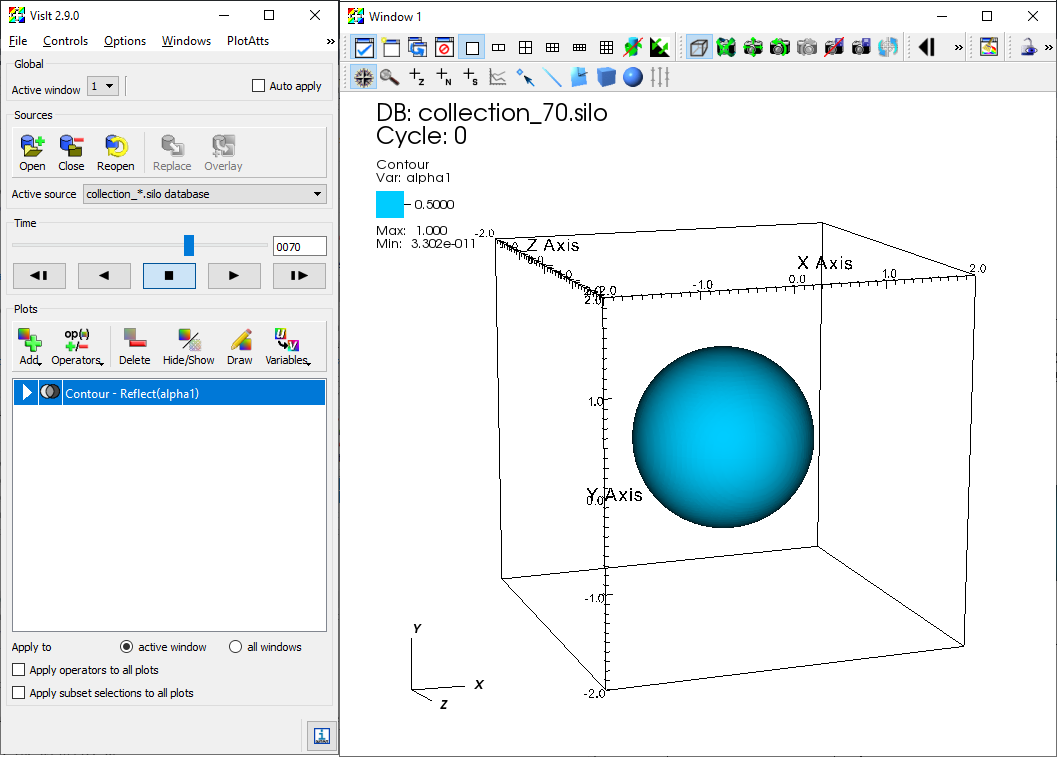
\includegraphics[width=\textwidth]{visit.png}
    \caption{Iso-contour of the liquid void fraction (\texttt{alpha1}) in the database generated by example case \texttt{3D_sphbubcollapse}.}
    \label{fig:visit} 
\end{figure}

\subsection{Serial data output}\label{s:serialdata}

If \texttt{parallel\_io = F} then MFC will output the conservative variables to a directory \texttt{D/}. 
If multiple cores are used ($\mathtt{ppn > 1}$) then a separate file is created for each core.
If there is only one coordinate dimension (\texttt{n = 0} and \texttt{p = 0}) then the primivative variables will also be written to \texttt{D/}.
The file names correspond to the variables associated with each equation solved by MFC.
They are written at every \texttt{t\_step\_save} time step.
The conservative variables are
\begin{gather}
    \{ (\rho \alpha)_1, \dots, (\rho\alpha)_{N_c}, \rho u_1, \dots, \rho u_{N_d}, E, \alpha_1, \dots, \alpha_{N_c} \},
\end{gather}
and the primitive variables are
\begin{gather}
    \{ (\rho \alpha)_1, \dots, (\rho\alpha)_{N_c}, u_1, \dots, u_{N_d}, p, \alpha_1, \dots, \alpha_{N_c} \},
\end{gather}
where $N_c$ are the number of components \texttt{num\_fluids} and $N_d$ is the number of spatial dimensions. 
There are exceptions: if \texttt{model\_eqns = 3}, then the six-equation model appends these variables with the internal energies of each component.
If there are sub-grid bubbles \texttt{bubbles = T}, then the bubble variables are also written. 
These depend on the bubble dynamics model used.
If \texttt{polytropic = T} then the conservative variables are appended by 
\begin{gather}
    \{ n_b R_1, n_b \Rdot_1, \dots, n_b R_{N_b}, n_b \Rdot_{N_b} \}
\end{gather}
where $n_B$ is the bubble number density and $N_b$ are the number of bubble sizes (see matching variable in the input file, \texttt{Nb}).
The primitive bubble variables do not include $n_B$:
\begin{gather}
    \{ R_1, \Rdot_1, \dots, R_{N_b}, \Rdot_{N_b} \}.
\end{gather}

\newpage
\section*{Acknowledgements} 

This work was supported in part by multiple past grants from the US National Institute of Health (NIH), the US Office of Naval Research (ONR), and the US National Science Foundation (NSF), as well as current NIH grant number P01-DK043881 and ONR grant numbers N0014-17-1-2676 and N0014-18-1-2625.
The computations presented here utilized the Extreme Science and Engineering Discovery Environment, which is supported under NSF grant number CTS120005.
K.M. acknowledges support from the Funai Foundation for Information Technology via the Overseas Scholarship.

\newpage
\bibliographystyle{apalike}
\bibliography{ref}

% -------------------------------------------------------------------------------------------------------------------
\newpage
\appendix

\section{Boundary conditions}\label{s:bcs}

\begin{table}[H]
	\centering
	{\tablefont
	\begin{tabular}{ | c | c | l | }
	\hline
		  & \textbf{\#} & \textbf{Description} \\
		\hline
		\parbox[t]{2.5mm}{\multirow{5}{*}{\rotatebox[origin=c]{90}{Normal}}} 
		& $-1$ & Periodic\\
		& $-2$ & Reflective\\
		& $-3$ & Ghost cell extrapolation \\
		& $-4$ & Riemann extrapolation \\
		& $-5$ & Slip wall \\
		\hline
		\parbox[t]{2.5mm}{\multirow{7}{*}{\rotatebox[origin=c]{90}{Characteristic.}}} 
		& $-6$ & Non-reflecting subsonic buffer \\
		& $-7$ & Non-reflecting subsonic inflow \\
		& $-8$ & Non-reflecting subsonic outflow \\
		& $-9$ & Force-free subsonic outflow \\
		& $-10$ & Constant pressure subsonic outflow \\
		& $-11$ & Supersonic inflow \\
		& $-12$ & Supersonic outflow \\
		\hline
	\end{tabular}}
	\caption{Boundary conditions.}
	\label{t:bcs}
\end{table}
	
The boundary condition supported by the MFC are listed in table~\ref{t:bcs}. Their number (\textbf{\#})
corresponds to the input value in \texttt{input.py} labeled \texttt{bc\_x[y,z]\%beg[end]} (see table~\ref{t:algorithm}).
The entries labeled ``Characteristic.'' are characteristic boundary conditions based on ~\citet{Thompson87}
and~\citet{Thompson90}.

\section{Patch types}\label{s:patches}

\begin{table}[H]
{\tablefont
	\centering
	\begin{tabularx}{\textwidth}{ | c |  l c c L | }
	\hline
		\textbf{\#} & \multicolumn{1}{c}{\bf Name} & \bf Dim. & \bf Smooth & \bf Description and required parameters  \\
		\hline
		1 & Line segment 	& 1 & N & 		Requires \texttt{x\_centroid} and \texttt{x\_length}. \\
		\hline
		2 & Circle 			& 2 & Y &  	Requires \texttt{x[y]\_centroid} and \texttt{radius}. \\
		3 & Rectangle 		& 2  & N & 	Coordinate-aligned. Requires \texttt{x[y]\_centroid} and \texttt{x[y]\_length}. \\
		4 & Sweep line 		& 2 & Y  & 	Not coordinate aligned. Requires \texttt{x[y]\_centroid} and \texttt{normal(i)}. \\
		5 & Ellipse 		& 2 & Y  & 	Requires \texttt{x[y]\_centroid} and \texttt{radii(i)}. \\
		6 & Vortex 		& 2 & N  & 	Isentropic flow disturbance. Requires \texttt{x[y]\_centroid} and \texttt{radius}. \\
		7 & 2D analytical 	& 2 & N & 	Assigns the primitive variables as analytical functions. \\
		\hline
		8 & Sphere 		& 3 & Y & 		Requires \texttt{x[y,z]\_centroid} and \texttt{radius}.\\
		9 & Cuboid 		& 3 & N & 		Coordinate-aligned. Requires \texttt{x[y,z]\_centroid} and \texttt{x[y,z]\_length}. \\
		10 & Cylinder 		& 3 & Y &  	Requires \texttt{x[y,z]\_centroid}, \texttt{radius}, and \texttt{x[y,z]\_length}. \\
		11 & Sweep plane 	& 3 & Y & 		Not coordinate-aligned. Requires \texttt{x[y,z]\_centroid} and \texttt{normal(i)}. \\
		12 & Ellipsoid 		& 3  & Y  & 	Requires \texttt{x[y,z]\_centroid} and \texttt{radii(i)}. \\
		13 & 3D analytical 	& 3 & N & 		Assigns the primitive variables as analytical functions.\\
	\hline
	\end{tabularx}}
	\caption{Patch geometries}
	\label{t:patches}
\end{table}

The patch types supported by the MFC are listed in table~\ref{t:patches}. This includes
types exclusive to one-, two-, and three-dimensional problems. The patch type number (\textbf{\#})
corresponds to the input value in \texttt{input.py} labeled  \texttt{patch\_icpp(j)\%geometry} where
\texttt{j} is the patch index. Each patch requires a different set of parameters, which are 
also listed in this table.

\section{Flux limiter}\label{s:fl}

\begin{table}[H]
    \centering
	{\tablefont
	\begin{tabular}{ | c |  l | }
	\hline
		\textbf{\#} & \bf Description  \\
		\hline
		1 & Minmod \\
		2 & MC \\
		3 & Ospre  \\
		4 & Superbee \\
		5 & Sweby \\
		6 & van Albada\\
		7 & van Leer\\
		\hline
	\end{tabular}}
	\caption{Flux limiter}
	\label{t:fl}
\end{table}

The flux limiters supported by the MFC are listed in table~\ref{t:fl}. Each limiter can be specified by specifying the value of \texttt{flux_lim}. Details of their implementations can be found in \citet{Meng16}.

\end{document}
